\documentclass[10pt]{article}\usepackage[margin=.55in]{geometry}\usepackage[T1]{fontenc}\usepackage{graphicx}\setlength{\parindent}{0pt}\setlength{\parskip}{5pt}\sloppy\begin{document}{\large solve4 pivot-row normalization}\par Task T-1448. 3 November 2026.\par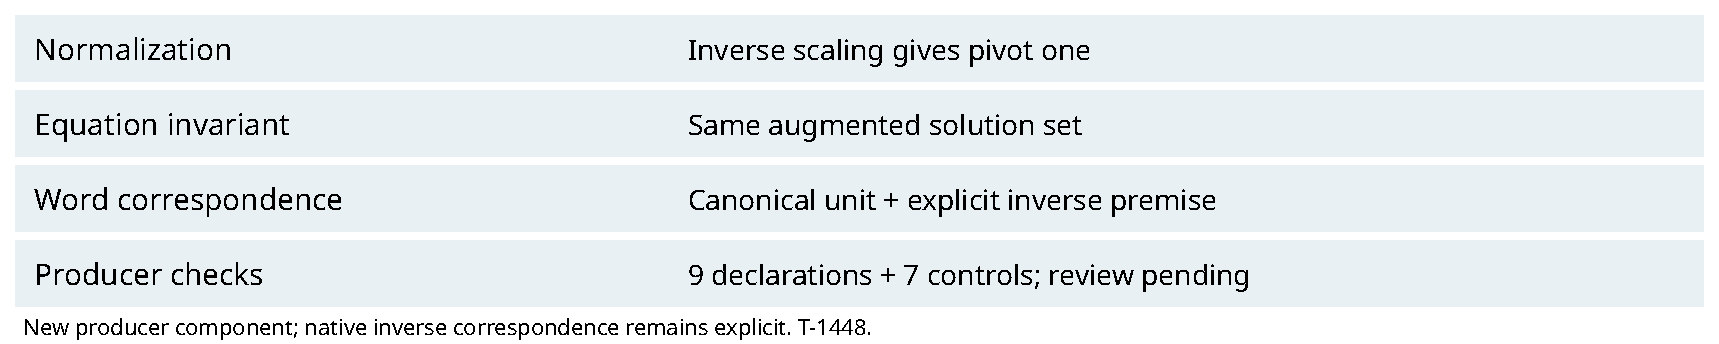
\includegraphics[width=\linewidth]{diagram.pdf}\par Nine declarations and seven exact controls passed, with 16 named axiom readbacks. The new field proof derives equation equivalence, pivot coefficient one and zero-prefix preservation for suffix scaling by the inverse of a nonzero pivot. The UInt64 contract transfers these conclusions under the existing canonical arithmetic bounds. This is producer evidence awaiting a new non-author source-fidelity review.

Native linkage. solve4 first selects and swaps a pivot row, computes unit=inv(mat[col][col],p) once, then multiplies entries j=col through 4, including the RHS. wordScale has this same row-value expression. Zero earlier coefficients make suffix scaling equal full-row scaling. The residual therefore scales by the unit; a nonzero unit preserves exactly the original solution set. The inverse of a nonzero field pivot supplies that unit and makes the pivot coefficient one. Prefix zeros are preserved.

Word contract. For prime p at most 2\textasciicircum{}32, canonical row entries and canonical unit make UInt64 multiplication decode to field multiplication. The theorem derives canonical output, preserved prefix, pivot one and equation equivalence for every solution vector. Native inv itself is not proved: the unit must be canonical and decode to the field inverse. The decoded pivot must be nonzero. These are arithmetic/input obligations, not assumed output equations. Search, swaps, array-loop semantics and complete solve4 correctness remain separate.

Controls and failures. The mod 7 row [0,2,4,0,6] with unit 4 becomes [0,1,2,0,3]; a nonvacuity theorem checks all inputs and derives the inverse identity by field cancellation from 4*2=1. Other controls check preserved solution, zero pivot, wrong unit, zero unit losing equation equivalence, and a nonzero prefix breaking suffix uniform scaling. A false wrong-unit theorem is rejected with exit 1. The first four attempts preserved fixture failures: arrow-row tokenization, opaque canonical decidability, nonreducing inverse computation and mismatched numeral/word-modulus field types. Failed controls exposed sorryAx and were rejected; none counted as accepted proof evidence. The nine theorem declarations compiled unchanged throughout.

Budget and verification. Five executed attempts used fixed 95-second ceilings under a prospectively amended maximum of six; the sixth was unused. The final passing attempt took 23.700560 seconds, all three children reaped, and 28,799 recursive input hashes stayed unchanged. Resources were 8 GiB address space,3500 MiB Lean heap,10 MiB OS stack,16 MiB Lean internal stack and one worker. Final axioms are only propext, Classical.choice and Quot.sound. Copied local helper source/oleans and shared upstream caches retain the disclosed Lean binary trust boundary; no independent binary/kernel checker was run. All failures and exact source revisions are archived.

Prior work. Nonzero row scaling is standard field algebra. Mathlib GroupWithZero.Basic documents inverse cancellation and the zero-inverse convention; the live documentation is background, while local hashed dependencies pin verification. The prior published suffix-elimination proof supplies Row, Vector, residual and word definitions. The present contribution connects the native normalization expression to the premises needed by that elimination proof.

Next construction. Prove the native modular exponentiation/inverse bridge, then derive the zero-prefix and nonzero-pivot inputs from selection, swapping and prior-column induction. The author of this packet authored the previous independent suffix review and cannot provide this packet's non-author fidelity verdict. No N19 cohort, matrix run, native trajectory, cloud computation or performance measurement was rerun.
\end{document}